%%% template.tex
%%%
%%% This LaTeX source document can be used as the basis for your technical
%%% paper or abstract. Regardless of the length of your document, the commands
%%% are all the same.
%%% 
%%% The "\documentclass" command is the first command in your file. If you want to 
%%% prepare a version of your article with line numbers - a "review" version - 
%%% include the "review" parameter:
%%%    \documentclass[review]{acmsiggraph}
%%%

\documentclass{acmsiggraph}

%%% Title of your article or abstract.

\title{Image Reconstructing with genetic Algorithms}

\author{Stephen N. Spencer\thanks{e-mail:spencer@cs.washington.edu}\\Chair, ACM SIGGRAPH Publications Committee}
\pdfauthor{Stephen N. Spencer}

%%% Used by the ``review'' variation; the online ID will be printed on 
%%% every page of the content.

\TOGonlineid{45678}

% User-generated keywords.

\keywords{radiosity, global illumination, constant time}

%%% The next five lines define the rights management block on the first page.
%%% Replace them with the LaTeX commands provided when the form has been completed.

\CopyrightYear{2016}
\setcopyright{acmcopyright}
\conferenceinfo{CONFERENCE PROGRAM NAME}{MONTH, DAY, and YEAR} 
\isbn{THIS-IS-A-SAMPLE-ISBN}\acmPrice{\$15.00}
\doi{http://doi.acm.org/THIS/IS/A/SAMPLE/DOI}

%%% Start of the document.

\begin{document}

%%% This is the ``teaser'' command, which puts an figure, centered, below 
%%% the title and author information, and above the body of the content.

 \teaser{
   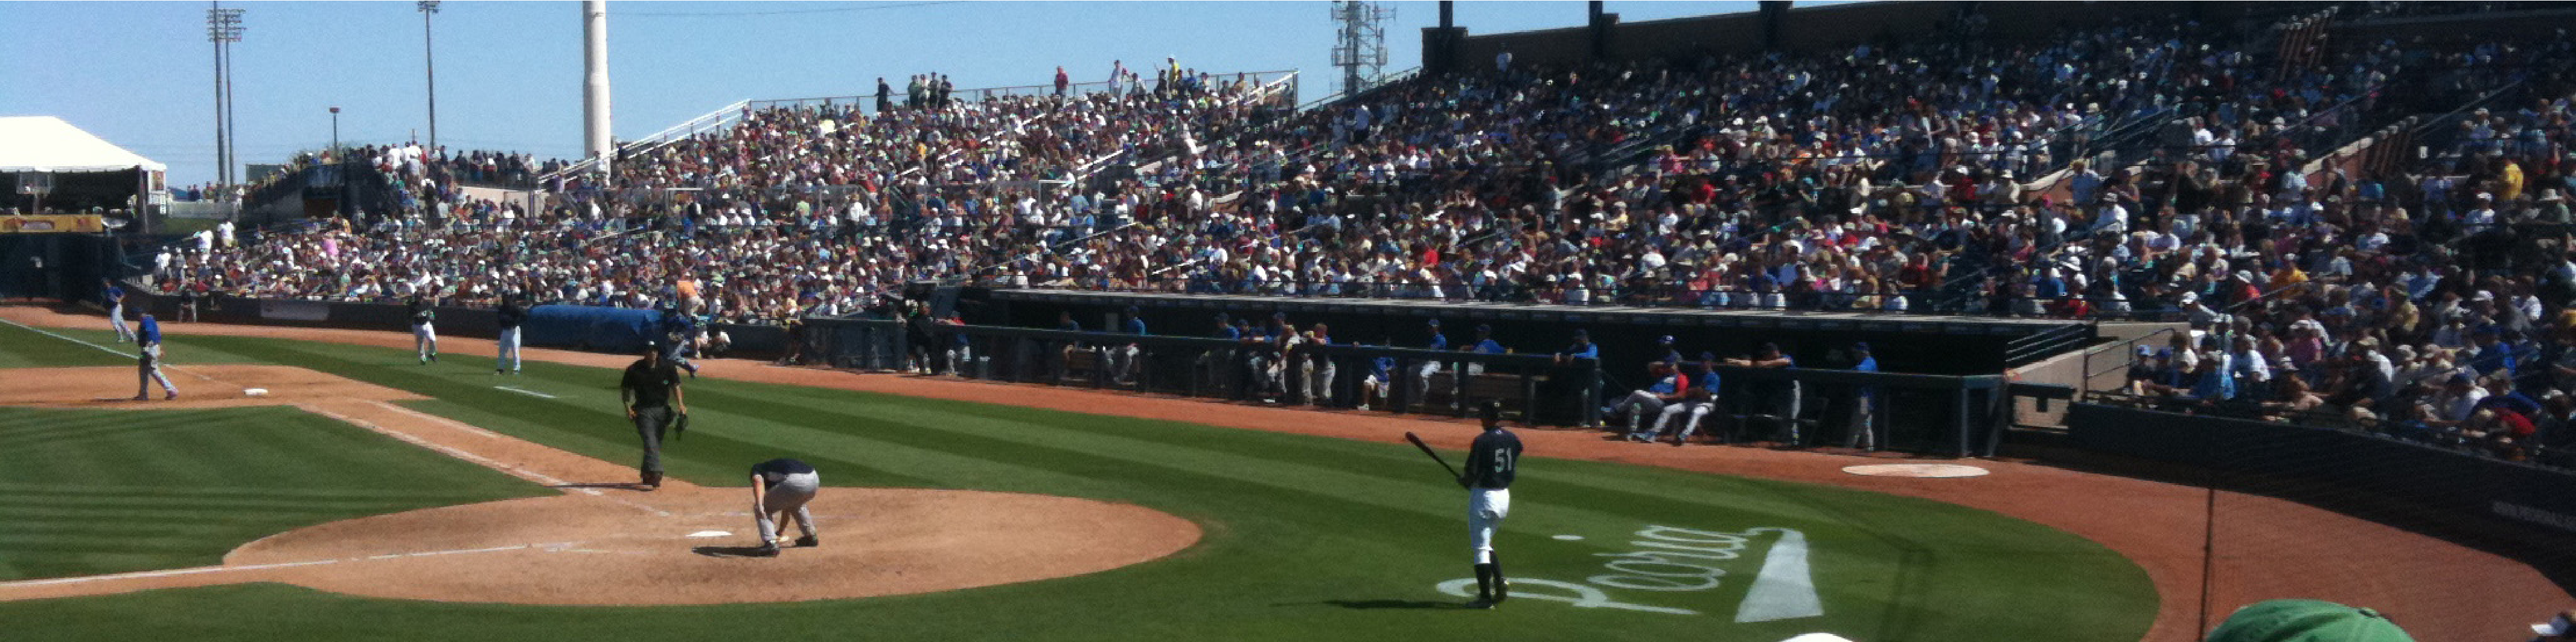
\includegraphics[height=1.5in]{images/sampleteaser}
   \caption{Spring Training 2009, Peoria, AZ.}
 }

\maketitle

\begin{abstract}

Abstract

\end{abstract}

%
% The code below should be generated by the tool at
% http://dl.acm.org/ccs.cfm
% Please copy and paste the code instead of the example below. 
%
\begin{CCSXML}
<ccs2012>
<concept>
<concept_id>10010147.10010371.10010382</concept_id>
<concept_desc>Computing methodologies~Image manipulation</concept_desc>
<concept_significance>500</concept_significance>
</concept>
<concept>
<concept_id>10010147.10010371.10010382.10010236</concept_id>
<concept_desc>Computing methodologies~Computational photography</concept_desc>
<concept_significance>300</concept_significance>
</concept>
</ccs2012>
\end{CCSXML}

\ccsdesc[500]{Computing methodologies~Image manipulation}
\ccsdesc[300]{Computing methodologies~Computational photography}

%
% End generated code
%

% The next three commands are required, and insert the user-generated keywords, 
% The CCS concepts list, and the rights management text.
% Please make sure there is a blank line between each of these three commands.

\keywordlist

\conceptlist

\printcopyright

\section{Concept}
\section{Genotype and Phenotype}
\section{Parent Selection}
\section{Convergence}



\section{Issues}


\begin{table}[ht]
  \centering
  \caption{A simple table.}
  \begin{tabular}{|r|l|}
    \hline
    7C0 & hexadecimal \\
    3700 & octal \\ \cline{2-2}
    11111000000 & binary \\
    \hline \hline
    1984 & decimal \\
    \hline
  \end{tabular}
\end{table}
  


\begin{figure}[ht]
  \centering
  \includegraphics[width=3.0in]{images/ferrari_laferrari}
  \caption{Ferrari LaFerrari. Image courtesy Flickr user ``gfreeman23.''}
  \label{fig:ferrari}
\end{figure}



\section*{Acknowledgements}

To Robert, for all the bagels.

\bibliographystyle{acmsiggraph}
\nocite{*}
\bibliography{template}
\end{document}
